\documentclass[1p]{elsarticle_modified}
%\bibliographystyle{elsarticle-num}

%\usepackage[colorlinks]{hyperref}
%\usepackage{abbrmath_seonhwa} %\Abb, \Ascr, \Acal ,\Abf, \Afrak
\usepackage{amsfonts}
\usepackage{amssymb}
\usepackage{amsmath}
\usepackage{amsthm}
\usepackage{scalefnt}
\usepackage{amsbsy}
\usepackage{kotex}
\usepackage{caption}
\usepackage{subfig}
\usepackage{color}
\usepackage{graphicx}
\usepackage{xcolor} %% white, black, red, green, blue, cyan, magenta, yellow
\usepackage{float}
\usepackage{setspace}
\usepackage{hyperref}

\usepackage{tikz}
\usetikzlibrary{arrows}

\usepackage{multirow}
\usepackage{array} % fixed length table
\usepackage{hhline}

%%%%%%%%%%%%%%%%%%%%%
\makeatletter
\renewcommand*\env@matrix[1][\arraystretch]{%
	\edef\arraystretch{#1}%
	\hskip -\arraycolsep
	\let\@ifnextchar\new@ifnextchar
	\array{*\c@MaxMatrixCols c}}
\makeatother %https://tex.stackexchange.com/questions/14071/how-can-i-increase-the-line-spacing-in-a-matrix
%%%%%%%%%%%%%%%

\usepackage[normalem]{ulem}

\newcommand{\msout}[1]{\ifmmode\text{\sout{\ensuremath{#1}}}\else\sout{#1}\fi}
%SOURCE: \msout is \stkout macro in https://tex.stackexchange.com/questions/20609/strikeout-in-math-mode

\newcommand{\cancel}[1]{
	\ifmmode
	{\color{red}\msout{#1}}
	\else
	{\color{red}\sout{#1}}
	\fi
}

\newcommand{\add}[1]{
	{\color{blue}\uwave{#1}}
}

\newcommand{\replace}[2]{
	\ifmmode
	{\color{red}\msout{#1}}{\color{blue}\uwave{#2}}
	\else
	{\color{red}\sout{#1}}{\color{blue}\uwave{#2}}
	\fi
}

\newcommand{\Sol}{\mathcal{S}} %segment
\newcommand{\D}{D} %diagram
\newcommand{\A}{\mathcal{A}} %arc


%%%%%%%%%%%%%%%%%%%%%%%%%%%%%5 test

\def\sl{\operatorname{\textup{SL}}(2,\Cbb)}
\def\psl{\operatorname{\textup{PSL}}(2,\Cbb)}
\def\quan{\mkern 1mu \triangleright \mkern 1mu}

\theoremstyle{definition}
\newtheorem{thm}{Theorem}[section]
\newtheorem{prop}[thm]{Proposition}
\newtheorem{lem}[thm]{Lemma}
\newtheorem{ques}[thm]{Question}
\newtheorem{cor}[thm]{Corollary}
\newtheorem{defn}[thm]{Definition}
\newtheorem{exam}[thm]{Example}
\newtheorem{rmk}[thm]{Remark}
\newtheorem{alg}[thm]{Algorithm}

\newcommand{\I}{\sqrt{-1}}
\begin{document}

%\begin{frontmatter}
%
%\title{Boundary parabolic representations of knots up to 8 crossings}
%
%%% Group authors per affiliation:
%\author{Yunhi Cho} 
%\address{Department of Mathematics, University of Seoul, Seoul, Korea}
%\ead{yhcho@uos.ac.kr}
%
%
%\author{Seonhwa Kim} %\fnref{s_kim}}
%\address{Center for Geometry and Physics, Institute for Basic Science, Pohang, 37673, Korea}
%\ead{ryeona17@ibs.re.kr}
%
%\author{Hyuk Kim}
%\address{Department of Mathematical Sciences, Seoul National University, Seoul 08826, Korea}
%\ead{hyukkim@snu.ac.kr}
%
%\author{Seokbeom Yoon}
%\address{Department of Mathematical Sciences, Seoul National University, Seoul, 08826,  Korea}
%\ead{sbyoon15@snu.ac.kr}
%
%\begin{abstract}
%We find all boundary parabolic representation of knots up to 8 crossings.
%
%\end{abstract}
%\begin{keyword}
%    \MSC[2010] 57M25 
%\end{keyword}
%
%\end{frontmatter}

%\linenumbers
%\tableofcontents
%
\newcommand\colored[1]{\textcolor{white}{\rule[-0.35ex]{0.8em}{1.4ex}}\kern-0.8em\color{red} #1}%
%\newcommand\colored[1]{\textcolor{white}{ #1}\kern-2.17ex	\textcolor{white}{ #1}\kern-1.81ex	\textcolor{white}{ #1}\kern-2.15ex\color{red}#1	}

{\Large $\underline{12n_{0870}~(K12n_{0870})}$}

\setlength{\tabcolsep}{10pt}
\renewcommand{\arraystretch}{1.6}
\vspace{1cm}\begin{tabular}{m{100pt}>{\centering\arraybackslash}m{274pt}}
\multirow{5}{120pt}{
	\centering
	\includegraphics[width=112pt]{../../../GIT/diagram.site/Diagrams/png/2959_12n_0870.png}\\
\ \ \ A knot diagram\footnotemark}&
\allowdisplaybreaks
\textbf{Linearized knot diagam} \\
\cline{2-2}
 &
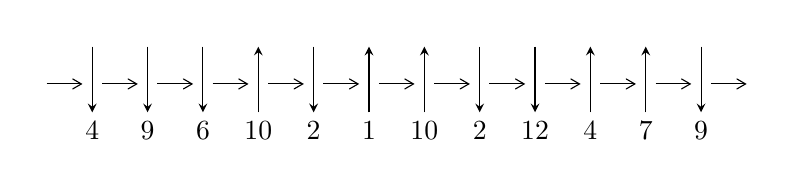
\begin{tikzpicture}[x=20pt, y=17pt]
	% nodes
	\node (C0) at (0, 0) {};
	\node (C1) at (1, 0) {};
	\node (C1U) at (1, +1) {};
	\node (C1D) at (1, -1) {4};

	\node (C2) at (2, 0) {};
	\node (C2U) at (2, +1) {};
	\node (C2D) at (2, -1) {9};

	\node (C3) at (3, 0) {};
	\node (C3U) at (3, +1) {};
	\node (C3D) at (3, -1) {6};

	\node (C4) at (4, 0) {};
	\node (C4U) at (4, +1) {};
	\node (C4D) at (4, -1) {10};

	\node (C5) at (5, 0) {};
	\node (C5U) at (5, +1) {};
	\node (C5D) at (5, -1) {2};

	\node (C6) at (6, 0) {};
	\node (C6U) at (6, +1) {};
	\node (C6D) at (6, -1) {1};

	\node (C7) at (7, 0) {};
	\node (C7U) at (7, +1) {};
	\node (C7D) at (7, -1) {10};

	\node (C8) at (8, 0) {};
	\node (C8U) at (8, +1) {};
	\node (C8D) at (8, -1) {2};

	\node (C9) at (9, 0) {};
	\node (C9U) at (9, +1) {};
	\node (C9D) at (9, -1) {12};

	\node (C10) at (10, 0) {};
	\node (C10U) at (10, +1) {};
	\node (C10D) at (10, -1) {4};

	\node (C11) at (11, 0) {};
	\node (C11U) at (11, +1) {};
	\node (C11D) at (11, -1) {7};

	\node (C12) at (12, 0) {};
	\node (C12U) at (12, +1) {};
	\node (C12D) at (12, -1) {9};
	\node (C13) at (13, 0) {};

	% arrows
	\draw[->,>={angle 60}]
	(C0) edge (C1) (C1) edge (C2) (C2) edge (C3) (C3) edge (C4) (C4) edge (C5) (C5) edge (C6) (C6) edge (C7) (C7) edge (C8) (C8) edge (C9) (C9) edge (C10) (C10) edge (C11) (C11) edge (C12) (C12) edge (C13) ;	\draw[->,>=stealth]
	(C1U) edge (C1D) (C2U) edge (C2D) (C3U) edge (C3D) (C4D) edge (C4U) (C5U) edge (C5D) (C6D) edge (C6U) (C7D) edge (C7U) (C8U) edge (C8D) (C9U) edge (C9D) (C10D) edge (C10U) (C11D) edge (C11U) (C12U) edge (C12D) ;
	\end{tikzpicture} \\
\hhline{~~} \\& 
\textbf{Solving Sequence} \\ \cline{2-2} 
 &
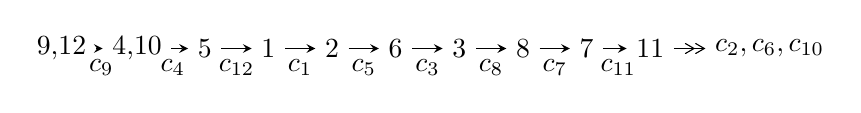
\begin{tikzpicture}[x=23pt, y=7pt]
	% node
	\node (A0) at (-1/8, 0) {9,12};
	\node (A1) at (17/16, 0) {4,10};
	\node (A2) at (17/8, 0) {5};
	\node (A3) at (25/8, 0) {1};
	\node (A4) at (33/8, 0) {2};
	\node (A5) at (41/8, 0) {6};
	\node (A6) at (49/8, 0) {3};
	\node (A7) at (57/8, 0) {8};
	\node (A8) at (65/8, 0) {7};
	\node (A9) at (73/8, 0) {11};
	\node (C1) at (1/2, -1) {$c_{9}$};
	\node (C2) at (13/8, -1) {$c_{4}$};
	\node (C3) at (21/8, -1) {$c_{12}$};
	\node (C4) at (29/8, -1) {$c_{1}$};
	\node (C5) at (37/8, -1) {$c_{5}$};
	\node (C6) at (45/8, -1) {$c_{3}$};
	\node (C7) at (53/8, -1) {$c_{8}$};
	\node (C8) at (61/8, -1) {$c_{7}$};
	\node (C9) at (69/8, -1) {$c_{11}$};
	\node (A10) at (11, 0) {$c_{2},c_{6},c_{10}$};

	% edge
	\draw[->,>=stealth]	
	(A0) edge (A1) (A1) edge (A2) (A2) edge (A3) (A3) edge (A4) (A4) edge (A5) (A5) edge (A6) (A6) edge (A7) (A7) edge (A8) (A8) edge (A9) ;
	\draw[->>,>={angle 60}]	
	(A9) edge (A10);
\end{tikzpicture} \\ 

\end{tabular} \\

\footnotetext{
The image of knot diagram is generated by the software ``\textbf{Draw programme}" developed by Andrew Bartholomew(\url{http://www.layer8.co.uk/maths/draw/index.htm\#Running-draw}), where we modified some parts for our purpose(\url{https://github.com/CATsTAILs/LinksPainter}).
}\phantom \\ \newline 
\centering \textbf{Ideals for irreducible components\footnotemark of $X_{\text{par}}$} 
 
\begin{align*}
I^u_{1}&=\langle 
-9.00164\times10^{56} u^{36}-3.79644\times10^{57} u^{35}+\cdots+2.25166\times10^{59} b-2.70335\times10^{59},\\
\phantom{I^u_{1}}&\phantom{= \langle  }3.91048\times10^{57} u^{36}+9.08535\times10^{57} u^{35}+\cdots+6.75498\times10^{59} a-7.61995\times10^{59},\;u^{37}+3 u^{36}+\cdots+27 u+27\rangle \\
I^u_{2}&=\langle 
-1131323800 u^{24}+8093044710 u^{23}+\cdots+3924483813 b+3811509091,\\
\phantom{I^u_{2}}&\phantom{= \langle  }6486714421 u^{24}-23913418584 u^{23}+\cdots+3924483813 a+14656680362,\\
\phantom{I^u_{2}}&\phantom{= \langle  }u^{25}-4 u^{24}+\cdots-9 u+1\rangle \\
\\
\end{align*}
\raggedright * 2 irreducible components of $\dim_{\mathbb{C}}=0$, with total 62 representations.\\
\footnotetext{All coefficients of polynomials are rational numbers. But the coefficients are sometimes approximated in decimal forms when there is not enough margin.}
\newpage
\renewcommand{\arraystretch}{1}
\centering \section*{I. $I^u_{1}= \langle -9.00\times10^{56} u^{36}-3.80\times10^{57} u^{35}+\cdots+2.25\times10^{59} b-2.70\times10^{59},\;3.91\times10^{57} u^{36}+9.09\times10^{57} u^{35}+\cdots+6.75\times10^{59} a-7.62\times10^{59},\;u^{37}+3 u^{36}+\cdots+27 u+27 \rangle$}
\flushleft \textbf{(i) Arc colorings}\\
\begin{tabular}{m{7pt} m{180pt} m{7pt} m{180pt} }
\flushright $a_{9}=$&$\begin{pmatrix}1\\0\end{pmatrix}$ \\
\flushright $a_{12}=$&$\begin{pmatrix}0\\u\end{pmatrix}$ \\
\flushright $a_{4}=$&$\begin{pmatrix}-0.00578904 u^{36}-0.0134499 u^{35}+\cdots-3.92304 u+1.12805\\0.00399778 u^{36}+0.0168606 u^{35}+\cdots-0.325413 u+1.20060\end{pmatrix}$ \\
\flushright $a_{10}=$&$\begin{pmatrix}1\\u^2\end{pmatrix}$ \\
\flushright $a_{5}=$&$\begin{pmatrix}-0.000411239 u^{36}+0.00236692 u^{35}+\cdots-4.29899 u+2.43442\\0.00328021 u^{36}+0.0148958 u^{35}+\cdots-0.462065 u+1.20915\end{pmatrix}$ \\
\flushright $a_{1}=$&$\begin{pmatrix}- u\\u\end{pmatrix}$ \\
\flushright $a_{2}=$&$\begin{pmatrix}-0.0189562 u^{36}-0.0588044 u^{35}+\cdots-1.78606 u-1.25542\\-0.00948539 u^{36}-0.0280353 u^{35}+\cdots-3.10510 u-0.162459\end{pmatrix}$ \\
\flushright $a_{6}=$&$\begin{pmatrix}0.0309726 u^{36}+0.0803799 u^{35}+\cdots+6.68023 u-0.585521\\-0.00665213 u^{36}-0.0225712 u^{35}+\cdots+0.785980 u-1.34064\end{pmatrix}$ \\
\flushright $a_{3}=$&$\begin{pmatrix}-0.00947083 u^{36}-0.0307691 u^{35}+\cdots+1.31904 u-1.09296\\-0.00948539 u^{36}-0.0280353 u^{35}+\cdots-3.10510 u-0.162459\end{pmatrix}$ \\
\flushright $a_{8}=$&$\begin{pmatrix}-0.0288137 u^{36}-0.0681602 u^{35}+\cdots-7.98371 u+2.22311\\0.00233006 u^{36}+0.00798065 u^{35}+\cdots-1.26663 u+1.55312\end{pmatrix}$ \\
\flushright $a_{7}=$&$\begin{pmatrix}-0.0301650 u^{36}-0.0794968 u^{35}+\cdots-6.43270 u+0.176402\\0.00584456 u^{36}+0.0216881 u^{35}+\cdots-1.03351 u+1.74976\end{pmatrix}$ \\
\flushright $a_{11}=$&$\begin{pmatrix}0.0207989 u^{36}+0.0467173 u^{35}+\cdots+6.44147 u-1.65281\\-0.0128462 u^{36}-0.0354139 u^{35}+\cdots-0.0326585 u-1.80165\end{pmatrix}$\\&\end{tabular}
\flushleft \textbf{(ii) Obstruction class $= -1$}\\~\\
\flushleft \textbf{(iii) Cusp Shapes $= 0.0119190 u^{36}+0.0677566 u^{35}+\cdots-7.20128 u-2.71469$}\\~\\
\newpage\renewcommand{\arraystretch}{1}
\flushleft \textbf{(iv) u-Polynomials at the component}\newline \\
\begin{tabular}{m{50pt}|m{274pt}}
Crossings & \hspace{64pt}u-Polynomials at each crossing \\
\hline $$\begin{aligned}c_{1}\end{aligned}$$&$\begin{aligned}
&u^{37}-4 u^{36}+\cdots-2323 u+371
\end{aligned}$\\
\hline $$\begin{aligned}c_{2},c_{8}\end{aligned}$$&$\begin{aligned}
&u^{37}+u^{36}+\cdots-73337 u+9059
\end{aligned}$\\
\hline $$\begin{aligned}c_{3}\end{aligned}$$&$\begin{aligned}
&u^{37}-3 u^{36}+\cdots-924 u+436
\end{aligned}$\\
\hline $$\begin{aligned}c_{4},c_{10}\end{aligned}$$&$\begin{aligned}
&u^{37}+u^{36}+\cdots+57272 u+22021
\end{aligned}$\\
\hline $$\begin{aligned}c_{5}\end{aligned}$$&$\begin{aligned}
&u^{37}-2 u^{36}+\cdots+26864 u+132947
\end{aligned}$\\
\hline $$\begin{aligned}c_{6}\end{aligned}$$&$\begin{aligned}
&u^{37}+4 u^{36}+\cdots+69 u+71
\end{aligned}$\\
\hline $$\begin{aligned}c_{7}\end{aligned}$$&$\begin{aligned}
&u^{37}+5 u^{36}+\cdots-90135 u+22247
\end{aligned}$\\
\hline $$\begin{aligned}c_{9},c_{12}\end{aligned}$$&$\begin{aligned}
&u^{37}-3 u^{36}+\cdots+27 u-27
\end{aligned}$\\
\hline $$\begin{aligned}c_{11}\end{aligned}$$&$\begin{aligned}
&u^{37}-2 u^{36}+\cdots+8266 u+347
\end{aligned}$\\
\hline
\end{tabular}\\~\\
\newpage\renewcommand{\arraystretch}{1}
\flushleft \textbf{(v) Riley Polynomials at the component}\newline \\
\begin{tabular}{m{50pt}|m{274pt}}
Crossings & \hspace{64pt}Riley Polynomials at each crossing \\
\hline $$\begin{aligned}c_{1}\end{aligned}$$&$\begin{aligned}
&y^{37}+12 y^{36}+\cdots-1418941 y-137641
\end{aligned}$\\
\hline $$\begin{aligned}c_{2},c_{8}\end{aligned}$$&$\begin{aligned}
&y^{37}+65 y^{36}+\cdots-1244302617 y-82065481
\end{aligned}$\\
\hline $$\begin{aligned}c_{3}\end{aligned}$$&$\begin{aligned}
&y^{37}+15 y^{36}+\cdots-3507096 y-190096
\end{aligned}$\\
\hline $$\begin{aligned}c_{4},c_{10}\end{aligned}$$&$\begin{aligned}
&y^{37}-63 y^{36}+\cdots-4284792146 y-484924441
\end{aligned}$\\
\hline $$\begin{aligned}c_{5}\end{aligned}$$&$\begin{aligned}
&y^{37}+84 y^{36}+\cdots-186496418056 y-17674904809
\end{aligned}$\\
\hline $$\begin{aligned}c_{6}\end{aligned}$$&$\begin{aligned}
&y^{37}-12 y^{36}+\cdots+153577 y-5041
\end{aligned}$\\
\hline $$\begin{aligned}c_{7}\end{aligned}$$&$\begin{aligned}
&y^{37}-79 y^{36}+\cdots-621600391 y-494929009
\end{aligned}$\\
\hline $$\begin{aligned}c_{9},c_{12}\end{aligned}$$&$\begin{aligned}
&y^{37}+35 y^{36}+\cdots-6075 y-729
\end{aligned}$\\
\hline $$\begin{aligned}c_{11}\end{aligned}$$&$\begin{aligned}
&y^{37}-16 y^{36}+\cdots+76266810 y-120409
\end{aligned}$\\
\hline
\end{tabular}\\~\\
\newpage\flushleft \textbf{(vi) Complex Volumes and Cusp Shapes}
$$\begin{array}{c|c|c}  
\text{Solutions to }I^u_{1}& \I (\text{vol} + \sqrt{-1}CS) & \text{Cusp shape}\\
 \hline 
\begin{aligned}
u &= -0.167576 + 1.059820 I \\
a &= -3.68479 + 0.47830 I \\
b &= \phantom{-}4.00168 - 0.78199 I\end{aligned}
 & -6.33270 + 0.58456 I & \phantom{-}4.48833 + 4.92922 I \\ \hline\begin{aligned}
u &= -0.167576 - 1.059820 I \\
a &= -3.68479 - 0.47830 I \\
b &= \phantom{-}4.00168 + 0.78199 I\end{aligned}
 & -6.33270 - 0.58456 I & \phantom{-}4.48833 - 4.92922 I \\ \hline\begin{aligned}
u &= -0.459153 + 1.191530 I \\
a &= \phantom{-}0.82442 - 1.37289 I \\
b &= -1.58984 + 0.88747 I\end{aligned}
 & \phantom{-}4.34687 + 6.37531 I & \phantom{-}4.85551 - 8.12342 I \\ \hline\begin{aligned}
u &= -0.459153 - 1.191530 I \\
a &= \phantom{-}0.82442 + 1.37289 I \\
b &= -1.58984 - 0.88747 I\end{aligned}
 & \phantom{-}4.34687 - 6.37531 I & \phantom{-}4.85551 + 8.12342 I \\ \hline\begin{aligned}
u &= -0.665909 + 0.256393 I \\
a &= \phantom{-}0.205806 - 1.100060 I \\
b &= -0.923196 - 0.122607 I\end{aligned}
 & \phantom{-}1.54386 - 2.11310 I & \phantom{-}0.69649 + 4.84319 I \\ \hline\begin{aligned}
u &= -0.665909 - 0.256393 I \\
a &= \phantom{-}0.205806 + 1.100060 I \\
b &= -0.923196 + 0.122607 I\end{aligned}
 & \phantom{-}1.54386 + 2.11310 I & \phantom{-}0.69649 - 4.84319 I \\ \hline\begin{aligned}
u &= \phantom{-}0.384563 + 1.236730 I \\
a &= \phantom{-}0.923969 + 0.381334 I \\
b &= -1.57334 - 0.01590 I\end{aligned}
 & \phantom{-}1.13766 - 4.82922 I & -4.75413 + 6.35770 I \\ \hline\begin{aligned}
u &= \phantom{-}0.384563 - 1.236730 I \\
a &= \phantom{-}0.923969 - 0.381334 I \\
b &= -1.57334 + 0.01590 I\end{aligned}
 & \phantom{-}1.13766 + 4.82922 I & -4.75413 - 6.35770 I \\ \hline\begin{aligned}
u &= -0.323724 + 1.264700 I \\
a &= \phantom{-}0.175356 - 0.423168 I \\
b &= \phantom{-}0.510942 - 0.182266 I\end{aligned}
 & \phantom{-}6.26009 + 0.98488 I & \phantom{-}1.65796 - 0.75056 I \\ \hline\begin{aligned}
u &= -0.323724 - 1.264700 I \\
a &= \phantom{-}0.175356 + 0.423168 I \\
b &= \phantom{-}0.510942 + 0.182266 I\end{aligned}
 & \phantom{-}6.26009 - 0.98488 I & \phantom{-}1.65796 + 0.75056 I\\
 \hline 
 \end{array}$$\newpage$$\begin{array}{c|c|c}  
\text{Solutions to }I^u_{1}& \I (\text{vol} + \sqrt{-1}CS) & \text{Cusp shape}\\
 \hline 
\begin{aligned}
u &= \phantom{-}0.385093 + 0.545017 I \\
a &= -0.268434 - 1.007740 I \\
b &= \phantom{-}0.185188 + 0.521817 I\end{aligned}
 & -0.024291 - 1.165760 I & -0.80928 + 6.18459 I \\ \hline\begin{aligned}
u &= \phantom{-}0.385093 - 0.545017 I \\
a &= -0.268434 + 1.007740 I \\
b &= \phantom{-}0.185188 - 0.521817 I\end{aligned}
 & -0.024291 + 1.165760 I & -0.80928 - 6.18459 I \\ \hline\begin{aligned}
u &= -0.061867 + 1.394640 I \\
a &= -0.984047 + 0.296932 I \\
b &= \phantom{-}0.406963 - 0.361276 I\end{aligned}
 & \phantom{-}13.74180 + 1.41481 I & \phantom{-}6.56734 - 5.56716 I \\ \hline\begin{aligned}
u &= -0.061867 - 1.394640 I \\
a &= -0.984047 - 0.296932 I \\
b &= \phantom{-}0.406963 + 0.361276 I\end{aligned}
 & \phantom{-}13.74180 - 1.41481 I & \phantom{-}6.56734 + 5.56716 I \\ \hline\begin{aligned}
u &= \phantom{-}0.567279 + 0.193554 I \\
a &= -0.42064 + 2.13487 I \\
b &= \phantom{-}0.585496 + 0.181304 I\end{aligned}
 & \phantom{-}0.41125 + 3.00174 I & -3.07390 - 3.64949 I \\ \hline\begin{aligned}
u &= \phantom{-}0.567279 - 0.193554 I \\
a &= -0.42064 - 2.13487 I \\
b &= \phantom{-}0.585496 - 0.181304 I\end{aligned}
 & \phantom{-}0.41125 - 3.00174 I & -3.07390 + 3.64949 I \\ \hline\begin{aligned}
u &= \phantom{-}0.322097 + 1.363570 I \\
a &= -0.809804 + 0.171126 I \\
b &= \phantom{-}1.48039 + 0.37445 I\end{aligned}
 & \phantom{-}3.14917 - 0.96903 I & \phantom{-0.000000 } 0 \\ \hline\begin{aligned}
u &= \phantom{-}0.322097 - 1.363570 I \\
a &= -0.809804 - 0.171126 I \\
b &= \phantom{-}1.48039 - 0.37445 I\end{aligned}
 & \phantom{-}3.14917 + 0.96903 I & \phantom{-0.000000 } 0 \\ \hline\begin{aligned}
u &= \phantom{-}0.481521 + 0.299204 I \\
a &= -0.29262 + 2.32677 I \\
b &= -0.287518 - 0.472642 I\end{aligned}
 & -1.88357 + 1.37786 I & -9.19174 + 1.54938 I \\ \hline\begin{aligned}
u &= \phantom{-}0.481521 - 0.299204 I \\
a &= -0.29262 - 2.32677 I \\
b &= -0.287518 + 0.472642 I\end{aligned}
 & -1.88357 - 1.37786 I & -9.19174 - 1.54938 I\\
 \hline 
 \end{array}$$\newpage$$\begin{array}{c|c|c}  
\text{Solutions to }I^u_{1}& \I (\text{vol} + \sqrt{-1}CS) & \text{Cusp shape}\\
 \hline 
\begin{aligned}
u &= \phantom{-}0.14297 + 1.43646 I \\
a &= -0.164059 + 0.136453 I \\
b &= -0.482858 + 0.065845 I\end{aligned}
 & \phantom{-}4.94395 - 5.26244 I & \phantom{-}4.95493 + 7.25561 I \\ \hline\begin{aligned}
u &= \phantom{-}0.14297 - 1.43646 I \\
a &= -0.164059 - 0.136453 I \\
b &= -0.482858 - 0.065845 I\end{aligned}
 & \phantom{-}4.94395 + 5.26244 I & \phantom{-}4.95493 - 7.25561 I \\ \hline\begin{aligned}
u &= -1.52010 + 0.15518 I \\
a &= \phantom{-}0.388678 + 0.524402 I \\
b &= -1.48572 + 0.39435 I\end{aligned}
 & \phantom{-}13.2585 + 5.7889 I & \phantom{-0.000000 } 0 \\ \hline\begin{aligned}
u &= -1.52010 - 0.15518 I \\
a &= \phantom{-}0.388678 - 0.524402 I \\
b &= -1.48572 - 0.39435 I\end{aligned}
 & \phantom{-}13.2585 - 5.7889 I & \phantom{-0.000000 } 0 \\ \hline\begin{aligned}
u &= -0.460772\phantom{ +0.000000I} \\
a &= \phantom{-}1.49046\phantom{ +0.000000I} \\
b &= \phantom{-}0.985143\phantom{ +0.000000I}\end{aligned}
 & -1.64677\phantom{ +0.000000I} & -6.24120\phantom{ +0.000000I} \\ \hline\begin{aligned}
u &= \phantom{-}1.14789 + 1.07616 I \\
a &= \phantom{-}0.290213 + 0.775019 I \\
b &= -1.39903 - 0.23170 I\end{aligned}
 & -5.26058 - 4.15697 I & \phantom{-}20.8250 + 0. I\phantom{ +0.000000I} \\ \hline\begin{aligned}
u &= \phantom{-}1.14789 - 1.07616 I \\
a &= \phantom{-}0.290213 - 0.775019 I \\
b &= -1.39903 + 0.23170 I\end{aligned}
 & -5.26058 + 4.15697 I & \phantom{-}20.8250 + 0. I\phantom{ +0.000000I} \\ \hline\begin{aligned}
u &= -0.129945 + 0.296598 I \\
a &= \phantom{-}1.42426 - 2.10190 I \\
b &= \phantom{-}1.58369 + 0.22057 I\end{aligned}
 & \phantom{-}9.68278 - 0.71257 I & -0.76102 - 2.68873 I \\ \hline\begin{aligned}
u &= -0.129945 - 0.296598 I \\
a &= \phantom{-}1.42426 + 2.10190 I \\
b &= \phantom{-}1.58369 - 0.22057 I\end{aligned}
 & \phantom{-}9.68278 + 0.71257 I & -0.76102 + 2.68873 I \\ \hline\begin{aligned}
u &= -0.06893 + 1.69284 I \\
a &= -2.11977 - 0.00511 I \\
b &= \phantom{-}3.07286 - 0.11340 I\end{aligned}
 & \phantom{-}17.2905 + 0.2066 I & \phantom{-0.000000 } 0\\
 \hline 
 \end{array}$$\newpage$$\begin{array}{c|c|c}  
\text{Solutions to }I^u_{1}& \I (\text{vol} + \sqrt{-1}CS) & \text{Cusp shape}\\
 \hline 
\begin{aligned}
u &= -0.06893 - 1.69284 I \\
a &= -2.11977 + 0.00511 I \\
b &= \phantom{-}3.07286 + 0.11340 I\end{aligned}
 & \phantom{-}17.2905 - 0.2066 I & \phantom{-0.000000 } 0 \\ \hline\begin{aligned}
u &= -0.65528 + 1.58363 I \\
a &= \phantom{-}1.13446 - 1.07747 I \\
b &= -2.20101 + 0.73181 I\end{aligned}
 & \phantom{-}18.6868 + 13.3663 I & \phantom{-0.000000 } 0 \\ \hline\begin{aligned}
u &= -0.65528 - 1.58363 I \\
a &= \phantom{-}1.13446 + 1.07747 I \\
b &= -2.20101 - 0.73181 I\end{aligned}
 & \phantom{-}18.6868 - 13.3663 I & \phantom{-0.000000 } 0 \\ \hline\begin{aligned}
u &= \phantom{-}0.22500 + 1.73667 I \\
a &= -1.55015 + 0.10298 I \\
b &= \phantom{-}2.47070 + 0.29718 I\end{aligned}
 & \phantom{-}7.62465 - 0.70239 I & \phantom{-0.000000 } 0 \\ \hline\begin{aligned}
u &= \phantom{-}0.22500 - 1.73667 I \\
a &= -1.55015 - 0.10298 I \\
b &= \phantom{-}2.47070 - 0.29718 I\end{aligned}
 & \phantom{-}7.62465 + 0.70239 I & \phantom{-0.000000 } 0 \\ \hline\begin{aligned}
u &= -0.87353 + 1.60469 I \\
a &= \phantom{-}0.515257 - 0.731056 I \\
b &= -0.347949 - 0.452043 I\end{aligned}
 & \phantom{-}17.5224 + 2.6853 I & \phantom{-0.000000 } 0 \\ \hline\begin{aligned}
u &= -0.87353 - 1.60469 I \\
a &= \phantom{-}0.515257 + 0.731056 I \\
b &= -0.347949 + 0.452043 I\end{aligned}
 & \phantom{-}17.5224 - 2.6853 I & \phantom{-0.000000 } 0\\
 \hline 
 \end{array}$$\newpage\newpage\renewcommand{\arraystretch}{1}
\centering \section*{II. $I^u_{2}= \langle -1.13\times10^{9} u^{24}+8.09\times10^{9} u^{23}+\cdots+3.92\times10^{9} b+3.81\times10^{9},\;6.49\times10^{9} u^{24}-2.39\times10^{10} u^{23}+\cdots+3.92\times10^{9} a+1.47\times10^{10},\;u^{25}-4 u^{24}+\cdots-9 u+1 \rangle$}
\flushleft \textbf{(i) Arc colorings}\\
\begin{tabular}{m{7pt} m{180pt} m{7pt} m{180pt} }
\flushright $a_{9}=$&$\begin{pmatrix}1\\0\end{pmatrix}$ \\
\flushright $a_{12}=$&$\begin{pmatrix}0\\u\end{pmatrix}$ \\
\flushright $a_{4}=$&$\begin{pmatrix}-1.65288 u^{24}+6.09339 u^{23}+\cdots-2.91819 u-3.73468\\0.288273 u^{24}-2.06219 u^{23}+\cdots+11.6354 u-0.971213\end{pmatrix}$ \\
\flushright $a_{10}=$&$\begin{pmatrix}1\\u^2\end{pmatrix}$ \\
\flushright $a_{5}=$&$\begin{pmatrix}-1.70636 u^{24}+5.59466 u^{23}+\cdots+11.7276 u-5.22403\\0.556721 u^{24}-2.37317 u^{23}+\cdots+5.27525 u-0.258587\end{pmatrix}$ \\
\flushright $a_{1}=$&$\begin{pmatrix}- u\\u\end{pmatrix}$ \\
\flushright $a_{2}=$&$\begin{pmatrix}-2.56378 u^{24}+7.61504 u^{23}+\cdots-28.4470 u+2.55259\\0.486242 u^{24}-1.35369 u^{23}+\cdots+3.80240 u-0.384318\end{pmatrix}$ \\
\flushright $a_{6}=$&$\begin{pmatrix}2.87677 u^{24}-11.8498 u^{23}+\cdots+78.7045 u-11.8129\\-0.240444 u^{24}+1.16517 u^{23}+\cdots-12.2022 u+1.62144\end{pmatrix}$ \\
\flushright $a_{3}=$&$\begin{pmatrix}-3.05002 u^{24}+8.96873 u^{23}+\cdots-32.2494 u+2.93691\\0.486242 u^{24}-1.35369 u^{23}+\cdots+3.80240 u-0.384318\end{pmatrix}$ \\
\flushright $a_{8}=$&$\begin{pmatrix}2.78473 u^{24}-11.4190 u^{23}+\cdots+69.1681 u-10.1842\\-0.363384 u^{24}+1.54406 u^{23}+\cdots-10.9514 u+1.76945\end{pmatrix}$ \\
\flushright $a_{7}=$&$\begin{pmatrix}2.73126 u^{24}-10.9178 u^{23}+\cdots+74.8139 u-11.6736\\-0.0949357 u^{24}+0.233088 u^{23}+\cdots-8.31152 u+1.48207\end{pmatrix}$ \\
\flushright $a_{11}=$&$\begin{pmatrix}3.25777 u^{24}-11.9300 u^{23}+\cdots+42.3975 u-3.58230\\-0.233376 u^{24}+1.03096 u^{23}+\cdots-10.7272 u+1.36206\end{pmatrix}$\\&\end{tabular}
\flushleft \textbf{(ii) Obstruction class $= 1$}\\~\\
\flushleft \textbf{(iii) Cusp Shapes $= \frac{16865762293}{3924483813} u^{24}-\frac{26283566834}{1308161271} u^{23}+\cdots+\frac{557421548465}{3924483813} u-\frac{84415101034}{3924483813}$}\\~\\
\newpage\renewcommand{\arraystretch}{1}
\flushleft \textbf{(iv) u-Polynomials at the component}\newline \\
\begin{tabular}{m{50pt}|m{274pt}}
Crossings & \hspace{64pt}u-Polynomials at each crossing \\
\hline $$\begin{aligned}c_{1}\end{aligned}$$&$\begin{aligned}
&u^{25}-7 u^{24}+\cdots+3 u-1
\end{aligned}$\\
\hline $$\begin{aligned}c_{2}\end{aligned}$$&$\begin{aligned}
&u^{25}+6 u^{23}+\cdots+u+1
\end{aligned}$\\
\hline $$\begin{aligned}c_{3}\end{aligned}$$&$\begin{aligned}
&u^{25}-6 u^{24}+\cdots+3 u-1
\end{aligned}$\\
\hline $$\begin{aligned}c_{4}\end{aligned}$$&$\begin{aligned}
&u^{25}-8 u^{23}+\cdots+8 u+1
\end{aligned}$\\
\hline $$\begin{aligned}c_{5}\end{aligned}$$&$\begin{aligned}
&u^{25}+3 u^{24}+\cdots-1944 u+631
\end{aligned}$\\
\hline $$\begin{aligned}c_{6}\end{aligned}$$&$\begin{aligned}
&u^{25}- u^{24}+\cdots-15 u+1
\end{aligned}$\\
\hline $$\begin{aligned}c_{7}\end{aligned}$$&$\begin{aligned}
&u^{25}+8 u^{24}+\cdots-2345 u-797
\end{aligned}$\\
\hline $$\begin{aligned}c_{8}\end{aligned}$$&$\begin{aligned}
&u^{25}+6 u^{23}+\cdots+u-1
\end{aligned}$\\
\hline $$\begin{aligned}c_{9}\end{aligned}$$&$\begin{aligned}
&u^{25}-4 u^{24}+\cdots-9 u+1
\end{aligned}$\\
\hline $$\begin{aligned}c_{10}\end{aligned}$$&$\begin{aligned}
&u^{25}-8 u^{23}+\cdots+8 u-1
\end{aligned}$\\
\hline $$\begin{aligned}c_{11}\end{aligned}$$&$\begin{aligned}
&u^{25}+u^{24}+\cdots+2 u-1
\end{aligned}$\\
\hline $$\begin{aligned}c_{12}\end{aligned}$$&$\begin{aligned}
&u^{25}+4 u^{24}+\cdots-9 u-1
\end{aligned}$\\
\hline
\end{tabular}\\~\\
\newpage\renewcommand{\arraystretch}{1}
\flushleft \textbf{(v) Riley Polynomials at the component}\newline \\
\begin{tabular}{m{50pt}|m{274pt}}
Crossings & \hspace{64pt}Riley Polynomials at each crossing \\
\hline $$\begin{aligned}c_{1}\end{aligned}$$&$\begin{aligned}
&y^{25}-5 y^{24}+\cdots+13 y-1
\end{aligned}$\\
\hline $$\begin{aligned}c_{2},c_{8}\end{aligned}$$&$\begin{aligned}
&y^{25}+12 y^{24}+\cdots-31 y-1
\end{aligned}$\\
\hline $$\begin{aligned}c_{3}\end{aligned}$$&$\begin{aligned}
&y^{25}-10 y^{24}+\cdots+15 y-1
\end{aligned}$\\
\hline $$\begin{aligned}c_{4},c_{10}\end{aligned}$$&$\begin{aligned}
&y^{25}-16 y^{24}+\cdots+24 y-1
\end{aligned}$\\
\hline $$\begin{aligned}c_{5}\end{aligned}$$&$\begin{aligned}
&y^{25}+7 y^{24}+\cdots+2558782 y-398161
\end{aligned}$\\
\hline $$\begin{aligned}c_{6}\end{aligned}$$&$\begin{aligned}
&y^{25}-5 y^{24}+\cdots-125 y-1
\end{aligned}$\\
\hline $$\begin{aligned}c_{7}\end{aligned}$$&$\begin{aligned}
&y^{25}-16 y^{24}+\cdots-2982649 y-635209
\end{aligned}$\\
\hline $$\begin{aligned}c_{9},c_{12}\end{aligned}$$&$\begin{aligned}
&y^{25}+18 y^{24}+\cdots+7 y-1
\end{aligned}$\\
\hline $$\begin{aligned}c_{11}\end{aligned}$$&$\begin{aligned}
&y^{25}+11 y^{24}+\cdots-12 y-1
\end{aligned}$\\
\hline
\end{tabular}\\~\\
\newpage\flushleft \textbf{(vi) Complex Volumes and Cusp Shapes}
$$\begin{array}{c|c|c}  
\text{Solutions to }I^u_{2}& \I (\text{vol} + \sqrt{-1}CS) & \text{Cusp shape}\\
 \hline 
\begin{aligned}
u &= -0.211608 + 0.978671 I \\
a &= \phantom{-}4.02880 - 1.31629 I \\
b &= -4.19783 + 0.93997 I\end{aligned}
 & -6.57774 + 0.83601 I & -12.6564 - 11.7355 I \\ \hline\begin{aligned}
u &= -0.211608 - 0.978671 I \\
a &= \phantom{-}4.02880 + 1.31629 I \\
b &= -4.19783 - 0.93997 I\end{aligned}
 & -6.57774 - 0.83601 I & -12.6564 + 11.7355 I \\ \hline\begin{aligned}
u &= -1.04938\phantom{ +0.000000I} \\
a &= -0.0313361\phantom{ +0.000000I} \\
b &= \phantom{-}1.39743\phantom{ +0.000000I}\end{aligned}
 & -0.108576\phantom{ +0.000000I} & \phantom{-}0.152620\phantom{ +0.000000I} \\ \hline\begin{aligned}
u &= \phantom{-}0.798599 + 0.744182 I \\
a &= -0.551742 - 1.128860 I \\
b &= \phantom{-}0.836085 - 0.082926 I\end{aligned}
 & \phantom{-}2.01196 + 0.69255 I & \phantom{-}1.79790 - 0.00493 I \\ \hline\begin{aligned}
u &= \phantom{-}0.798599 - 0.744182 I \\
a &= -0.551742 + 1.128860 I \\
b &= \phantom{-}0.836085 + 0.082926 I\end{aligned}
 & \phantom{-}2.01196 - 0.69255 I & \phantom{-}1.79790 + 0.00493 I \\ \hline\begin{aligned}
u &= \phantom{-}0.501731 + 0.720411 I \\
a &= -0.249121 + 1.158170 I \\
b &= -0.568048 - 0.400869 I\end{aligned}
 & -1.84833 - 2.11157 I & -3.19865 + 3.94763 I \\ \hline\begin{aligned}
u &= \phantom{-}0.501731 - 0.720411 I \\
a &= -0.249121 - 1.158170 I \\
b &= -0.568048 + 0.400869 I\end{aligned}
 & -1.84833 + 2.11157 I & -3.19865 - 3.94763 I \\ \hline\begin{aligned}
u &= \phantom{-}0.209489 + 1.126730 I \\
a &= \phantom{-}0.157093 - 0.519084 I \\
b &= -1.141540 + 0.622781 I\end{aligned}
 & \phantom{-}3.06603 - 4.36373 I & \phantom{-}1.36746 + 3.83070 I \\ \hline\begin{aligned}
u &= \phantom{-}0.209489 - 1.126730 I \\
a &= \phantom{-}0.157093 + 0.519084 I \\
b &= -1.141540 - 0.622781 I\end{aligned}
 & \phantom{-}3.06603 + 4.36373 I & \phantom{-}1.36746 - 3.83070 I \\ \hline\begin{aligned}
u &= \phantom{-}0.103688 + 0.826073 I \\
a &= \phantom{-}1.21034 + 1.47977 I \\
b &= \phantom{-}0.314331 - 0.723879 I\end{aligned}
 & \phantom{-}1.76724 + 3.08166 I & \phantom{-}2.11503 - 3.41199 I\\
 \hline 
 \end{array}$$\newpage$$\begin{array}{c|c|c}  
\text{Solutions to }I^u_{2}& \I (\text{vol} + \sqrt{-1}CS) & \text{Cusp shape}\\
 \hline 
\begin{aligned}
u &= \phantom{-}0.103688 - 0.826073 I \\
a &= \phantom{-}1.21034 - 1.47977 I \\
b &= \phantom{-}0.314331 + 0.723879 I\end{aligned}
 & \phantom{-}1.76724 - 3.08166 I & \phantom{-}2.11503 + 3.41199 I \\ \hline\begin{aligned}
u &= \phantom{-}0.535937 + 1.071200 I \\
a &= -0.690754 - 1.148390 I \\
b &= \phantom{-}1.67707 + 0.86201 I\end{aligned}
 & \phantom{-}3.25606 - 5.74154 I & -0.57302 + 3.73990 I \\ \hline\begin{aligned}
u &= \phantom{-}0.535937 - 1.071200 I \\
a &= -0.690754 + 1.148390 I \\
b &= \phantom{-}1.67707 - 0.86201 I\end{aligned}
 & \phantom{-}3.25606 + 5.74154 I & -0.57302 - 3.73990 I \\ \hline\begin{aligned}
u &= -0.318864 + 0.683122 I \\
a &= -0.054095 + 0.536492 I \\
b &= -1.59233 - 0.00324 I\end{aligned}
 & \phantom{-}9.97950 + 1.46375 I & \phantom{-}3.71841 - 5.95020 I \\ \hline\begin{aligned}
u &= -0.318864 - 0.683122 I \\
a &= -0.054095 - 0.536492 I \\
b &= -1.59233 + 0.00324 I\end{aligned}
 & \phantom{-}9.97950 - 1.46375 I & \phantom{-}3.71841 + 5.95020 I \\ \hline\begin{aligned}
u &= -0.510417 + 1.288240 I \\
a &= -0.87810 + 1.16015 I \\
b &= \phantom{-}1.43360 - 0.55061 I\end{aligned}
 & \phantom{-}4.00523 + 5.32915 I & \phantom{-}1.41990 - 1.29007 I \\ \hline\begin{aligned}
u &= -0.510417 - 1.288240 I \\
a &= -0.87810 - 1.16015 I \\
b &= \phantom{-}1.43360 + 0.55061 I\end{aligned}
 & \phantom{-}4.00523 - 5.32915 I & \phantom{-}1.41990 + 1.29007 I \\ \hline\begin{aligned}
u &= -0.16459 + 1.42006 I \\
a &= \phantom{-}1.178580 - 0.185673 I \\
b &= -0.815305 - 0.153731 I\end{aligned}
 & \phantom{-}13.10510 + 0.67738 I & -0.354087 + 0.858492 I \\ \hline\begin{aligned}
u &= -0.16459 - 1.42006 I \\
a &= \phantom{-}1.178580 + 0.185673 I \\
b &= -0.815305 + 0.153731 I\end{aligned}
 & \phantom{-}13.10510 - 0.67738 I & -0.354087 - 0.858492 I \\ \hline\begin{aligned}
u &= \phantom{-}0.20160 + 1.49559 I \\
a &= \phantom{-}0.529194 - 0.551861 I \\
b &= -0.710252 + 0.710457 I\end{aligned}
 & \phantom{-}4.43285 - 4.32284 I & \phantom{-}0.666667 + 0.650947 I\\
 \hline 
 \end{array}$$\newpage$$\begin{array}{c|c|c}  
\text{Solutions to }I^u_{2}& \I (\text{vol} + \sqrt{-1}CS) & \text{Cusp shape}\\
 \hline 
\begin{aligned}
u &= \phantom{-}0.20160 - 1.49559 I \\
a &= \phantom{-}0.529194 + 0.551861 I \\
b &= -0.710252 - 0.710457 I\end{aligned}
 & \phantom{-}4.43285 + 4.32284 I & \phantom{-}0.666667 - 0.650947 I \\ \hline\begin{aligned}
u &= \phantom{-}1.15413 + 1.05672 I \\
a &= \phantom{-}0.254363 + 0.770568 I \\
b &= -1.372110 - 0.235434 I\end{aligned}
 & -5.39972 - 4.16553 I & -36.8997 + 7.0211 I \\ \hline\begin{aligned}
u &= \phantom{-}1.15413 - 1.05672 I \\
a &= \phantom{-}0.254363 - 0.770568 I \\
b &= -1.372110 + 0.235434 I\end{aligned}
 & -5.39972 + 4.16553 I & -36.8997 - 7.0211 I \\ \hline\begin{aligned}
u &= \phantom{-}0.224993 + 0.114423 I \\
a &= -4.41889 - 1.18595 I \\
b &= \phantom{-}0.437604 + 0.274587 I\end{aligned}
 & -1.42493 - 1.96110 I & -1.97977 + 5.53360 I \\ \hline\begin{aligned}
u &= \phantom{-}0.224993 - 0.114423 I \\
a &= -4.41889 + 1.18595 I \\
b &= \phantom{-}0.437604 - 0.274587 I\end{aligned}
 & -1.42493 + 1.96110 I & -1.97977 - 5.53360 I\\
 \hline 
 \end{array}$$\newpage
\newpage\renewcommand{\arraystretch}{1}
\centering \section*{ III. u-Polynomials}
\begin{tabular}{m{50pt}|m{274pt}}
Crossings & \hspace{64pt}u-Polynomials at each crossing \\
\hline $$\begin{aligned}c_{1}\end{aligned}$$&$\begin{aligned}
&(u^{25}-7 u^{24}+\cdots+3 u-1)(u^{37}-4 u^{36}+\cdots-2323 u+371)
\end{aligned}$\\
\hline $$\begin{aligned}c_{2}\end{aligned}$$&$\begin{aligned}
&(u^{25}+6 u^{23}+\cdots+u+1)(u^{37}+u^{36}+\cdots-73337 u+9059)
\end{aligned}$\\
\hline $$\begin{aligned}c_{3}\end{aligned}$$&$\begin{aligned}
&(u^{25}-6 u^{24}+\cdots+3 u-1)(u^{37}-3 u^{36}+\cdots-924 u+436)
\end{aligned}$\\
\hline $$\begin{aligned}c_{4}\end{aligned}$$&$\begin{aligned}
&(u^{25}-8 u^{23}+\cdots+8 u+1)(u^{37}+u^{36}+\cdots+57272 u+22021)
\end{aligned}$\\
\hline $$\begin{aligned}c_{5}\end{aligned}$$&$\begin{aligned}
&(u^{25}+3 u^{24}+\cdots-1944 u+631)\\
&\cdot(u^{37}-2 u^{36}+\cdots+26864 u+132947)
\end{aligned}$\\
\hline $$\begin{aligned}c_{6}\end{aligned}$$&$\begin{aligned}
&(u^{25}- u^{24}+\cdots-15 u+1)(u^{37}+4 u^{36}+\cdots+69 u+71)
\end{aligned}$\\
\hline $$\begin{aligned}c_{7}\end{aligned}$$&$\begin{aligned}
&(u^{25}+8 u^{24}+\cdots-2345 u-797)(u^{37}+5 u^{36}+\cdots-90135 u+22247)
\end{aligned}$\\
\hline $$\begin{aligned}c_{8}\end{aligned}$$&$\begin{aligned}
&(u^{25}+6 u^{23}+\cdots+u-1)(u^{37}+u^{36}+\cdots-73337 u+9059)
\end{aligned}$\\
\hline $$\begin{aligned}c_{9}\end{aligned}$$&$\begin{aligned}
&(u^{25}-4 u^{24}+\cdots-9 u+1)(u^{37}-3 u^{36}+\cdots+27 u-27)
\end{aligned}$\\
\hline $$\begin{aligned}c_{10}\end{aligned}$$&$\begin{aligned}
&(u^{25}-8 u^{23}+\cdots+8 u-1)(u^{37}+u^{36}+\cdots+57272 u+22021)
\end{aligned}$\\
\hline $$\begin{aligned}c_{11}\end{aligned}$$&$\begin{aligned}
&(u^{25}+u^{24}+\cdots+2 u-1)(u^{37}-2 u^{36}+\cdots+8266 u+347)
\end{aligned}$\\
\hline $$\begin{aligned}c_{12}\end{aligned}$$&$\begin{aligned}
&(u^{25}+4 u^{24}+\cdots-9 u-1)(u^{37}-3 u^{36}+\cdots+27 u-27)
\end{aligned}$\\
\hline
\end{tabular}\newpage\renewcommand{\arraystretch}{1}
\centering \section*{ IV. Riley Polynomials}
\begin{tabular}{m{50pt}|m{274pt}}
Crossings & \hspace{64pt}Riley Polynomials at each crossing \\
\hline $$\begin{aligned}c_{1}\end{aligned}$$&$\begin{aligned}
&(y^{25}-5 y^{24}+\cdots+13 y-1)(y^{37}+12 y^{36}+\cdots-1418941 y-137641)
\end{aligned}$\\
\hline $$\begin{aligned}c_{2},c_{8}\end{aligned}$$&$\begin{aligned}
&(y^{25}+12 y^{24}+\cdots-31 y-1)\\
&\cdot(y^{37}+65 y^{36}+\cdots-1244302617 y-82065481)
\end{aligned}$\\
\hline $$\begin{aligned}c_{3}\end{aligned}$$&$\begin{aligned}
&(y^{25}-10 y^{24}+\cdots+15 y-1)\\
&\cdot(y^{37}+15 y^{36}+\cdots-3507096 y-190096)
\end{aligned}$\\
\hline $$\begin{aligned}c_{4},c_{10}\end{aligned}$$&$\begin{aligned}
&(y^{25}-16 y^{24}+\cdots+24 y-1)\\
&\cdot(y^{37}-63 y^{36}+\cdots-4284792146 y-484924441)
\end{aligned}$\\
\hline $$\begin{aligned}c_{5}\end{aligned}$$&$\begin{aligned}
&(y^{25}+7 y^{24}+\cdots+2558782 y-398161)\\
&\cdot(y^{37}+84 y^{36}+\cdots-186496418056 y-17674904809)
\end{aligned}$\\
\hline $$\begin{aligned}c_{6}\end{aligned}$$&$\begin{aligned}
&(y^{25}-5 y^{24}+\cdots-125 y-1)(y^{37}-12 y^{36}+\cdots+153577 y-5041)
\end{aligned}$\\
\hline $$\begin{aligned}c_{7}\end{aligned}$$&$\begin{aligned}
&(y^{25}-16 y^{24}+\cdots-2982649 y-635209)\\
&\cdot(y^{37}-79 y^{36}+\cdots-621600391 y-494929009)
\end{aligned}$\\
\hline $$\begin{aligned}c_{9},c_{12}\end{aligned}$$&$\begin{aligned}
&(y^{25}+18 y^{24}+\cdots+7 y-1)(y^{37}+35 y^{36}+\cdots-6075 y-729)
\end{aligned}$\\
\hline $$\begin{aligned}c_{11}\end{aligned}$$&$\begin{aligned}
&(y^{25}+11 y^{24}+\cdots-12 y-1)\\
&\cdot(y^{37}-16 y^{36}+\cdots+76266810 y-120409)
\end{aligned}$\\
\hline
\end{tabular}
\vskip 2pc
\end{document}